% Created 2018-02-15 Thu 18:45
\documentclass[11pt]{article}
\usepackage[utf8]{inputenc}
\usepackage[T1]{fontenc}
\usepackage{fixltx2e}
\usepackage{graphicx}
\usepackage{longtable}
\usepackage{float}
\usepackage{wrapfig}
\usepackage{rotating}
\usepackage[normalem]{ulem}
\usepackage{amsmath}
\usepackage{textcomp}
\usepackage{marvosym}
\usepackage{wasysym}
\usepackage{amssymb}
\usepackage{hyperref}
\tolerance=1000
\usepackage[pdftex]{insdljs}
\newcommand{\aDE}[4]{\begin{center}\begin{equation}\label{#4}\frac{{dy(t)}}{{dt}} -#1y(t) = #2u(t),y(0) = #3 \end{equation}\end{center}}
\newcommand\tugHello{Hello World!}
\begin{insDLJS}{mydljs}{My Private DLJS}function HelloWorld() {app.alert("\tugHello", 3); }\end{insDLJS}
\author{Changyuan Lin}
\date{\today}
\title{Test}
\hypersetup{
  pdfkeywords={},
  pdfsubject={},
  pdfcreator={Emacs 25.3.1 (Org mode 8.2.10)}}
\begin{document}

\maketitle
\tableofcontents

\section{Chapter 2}
\label{sec-1}
\subsection{JavaScript}
\label{sec-1-1}
\subsection{Answer Sheet via Email}
\label{sec-1-2}

\begin{Form}[action=mailto:forms@stackexchange.invalid?subject={CHE576HW02}&body=token,method=post]
    \noindent\TextField[stuid=stuid]{Student ID:}\\[1mm]
    \noindent\TextField[token=token]{token:}\\[1mm]
    \noindent\TextField[token=token]{token:}\\[1mm]
    \noindent\TextField[Q1=Q1]{Question1:}\\[1mm]
    \Reset{Reset} \quad \Submit{Submit} \quad 
\end{Form}


\begin{Form}[action=mailto:forms@stackexchange.invalid?subject={CHE576HW02}&body=token,method=post]
    \noindent\TextField[stuid=stuid]{Student ID:}\\[1mm]
    \noindent\TextField[token=token]{token:}\\[1mm]
    \noindent\TextField[token=token]{token:}\\[1mm]
    \noindent\TextField[Q1=Q1]{Question1:}\\[1mm]
    \Reset{Reset} \quad \Submit{Submit} \quad 
\end{Form}

\subsection{Answer Sheet via Post}
\label{sec-1-3}
\begin{Form}[action=mailto:forms@stackexchange.invalid?subject={The submitted form},method=post]
    \noindent\TextField[name=name]{Name:}\\[1mm]
    \ChoiceMenu[radio,name=gender]{Gender:}{male=male,female=fem}\\[1mm]
    \TextField[name=email,width=5cm]{E-mail:}\\[5mm]
    \Reset{Reset} \quad \Submit{Submit} \quad  \Acrobatmenu{Print}{Print}
\end{Form}
\subsection{ditaa \& \LaTeX{} Graph}
\label{sec-1-4}
For the physical process of tank dynamics given in the Figure below:

\vspace{0.2in}
\setlength{\unitlength}{1cm}
\begin{picture}(1, 1)
  \put(5, 0.9){\vector(1, 0){1.8}}
  \put(6.8, 0.9){\vector(0,-1){0.7}}
  \put(5.5,1.1){{$f_{in}(t)$}}   
  \put(6.3, 0.25){\line(0,-1){1.9}}
  \put(8.2, 0.25){\line(0,-1){1.9}}
  \put(6.3,-1.95){\framebox(1.9,1.9)}
  \put(8., -1.95){\vector(1,0){2.5}}  
  \put(9.6, -2.1){\line(0,0){0.4}}  
  \put(9.3, -2.1){\line(0,0){0.4}}  
  \put(9.3, -2.1){\line(3,4){0.3}}  
  \put(9.3, -1.75){\line(3,-4){0.3}}  
  \put(9.45,-2.){\line(0,1){0.5}}
  \put(9.15,-1.5){\line(1,0){0.5}}
   \put(10.7,-2){{$f_{out}(t)$}}  
   \put(9.3,-1.25){{$K$}}  
    \put(5.5,-1.25){{$h(t)$}}  
\end{picture}
\vspace{0.7in}


Solution:
\begin{itemize}
\item \( \frac{dh}{dt} = -\frac{1}{K\overline{A}}h + \frac{1}{\overline{A}}f_{in}\)
\item Assume that the tank height is measured, \(y(t) = h(t)\)
       \[\Sigma(A,B,C,D) = \Sigma\left(-\frac{1}{K\overline{A}}, \frac{1}{\overline{A}}, 1, 0\right)\]
\item The state-space realization is given as:
\end{itemize}

\begin{figure}[!htpb]
\centering
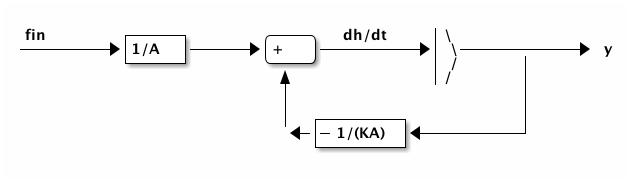
\includegraphics[width=3in,height=1.5in]{2222.png}
{\caption{Block diagram elements.}}
\end{figure}

\begin{itemize}
\item \[\begin{array}{c}
        \Phi = e^{-\frac{0.2}{K\overline{A}}}, \quad \Gamma = -K\left(e^{-\frac{0.2}{K\overline{A}}} - 1\right), \quad \theta = 1 \\[0.5cm]
        \Sigma(A_{d},B_{d},C_{d},D_{d}) = \Sigma\left( e^{-\frac{0.2}{K\overline{A}}}, -K\left(e^{-\frac{0.2}{K\overline{A}}} - 1\right), 1, 0\right)
        \end{array}\]
\item Assume that \(h(0) = 0\). Laplace transform:
\[ \frac{Y(s)}{U(s)} = \frac{5}{s+1}\]
\[\boxed{ \nonumber  \tau = 1, \quad \tau_{d} = 0\Rightarrow \Delta t = (0.1\sim0.2)1\tau = 0.1\sim 0.2}\]
\end{itemize}
% Emacs 25.3.1 (Org mode 8.2.10)
\end{document}
